\documentclass[handout,10pt]{beamer}
\usepackage[english, french]{babel}
%\usepackage[T1]{fontenc}
\usepackage{aeguill}
\usepackage[utf8]{inputenc}
\usepackage{amsmath}
\usepackage{graphicx}
\usepackage{xspace}
\usepackage{eurosym}
\usepackage{array}
\usepackage{handoutWithNotes}
\usepackage{soul}
\usepackage{hyperref}

%\pgfpagesuselayout{1 on 1 with notes}[a4paper,border shrink=5mm]

\usetheme{Darmstadt}
\usecolortheme{seahorse}

\newcommand{\etal}{\emph{et~al.}\xspace}
\newcommand{\vstrike}[1]{\ensuremath{\text{#1}\hspace{-.5em}|\hspace{.2em}}\xspace}

\setbeamertemplate{footline}{
\leavevmode%
\hbox{\hspace*{-0.06cm}
\begin{beamercolorbox}[wd=.2\paperwidth,ht=2.25ex,dp=1ex,center]{title in head/foot}%
  \usebeamerfont{author in head/foot}\insertshortauthor%~~(\insertshortinstitute)
\end{beamercolorbox}%
\begin{beamercolorbox}[wd=.6\paperwidth,ht=2.25ex,dp=1ex,center]{title in head/foot}%
  \usebeamerfont{section in head/foot}\insertshorttitle
\end{beamercolorbox}%
\begin{beamercolorbox}[wd=.2\paperwidth,ht=2.25ex,dp=1ex,right]{title in head/foot}%
  %\usebeamerfont{section in head/foot}\insertshortdate{}\hspace*{2em}
  \insertframenumber{} / \inserttotalframenumber\hspace*{2ex}
\end{beamercolorbox}}%
\vskip0pt%
}

%\definecolor{darkgreen}{rgb}{0,0.5,0}

\title{Tor~: routage et chiffrement en oignon}

%\author[GP]{Guillaume Piolle}
\author[Guillaume Piolle]{Guillaume Piolle\\\texttt{guillaume.piolle@supelec.fr}\\\texttt{http://guillaume.piolle.fr/}}

\institute{\includegraphics[width=2cm]{inc/cc-by}\\\href{http://creativecommons.org/licenses/by/4.0/}{Creative Commons Attribution 4.0}}
    
%\date[\today]{\today}
%\date{2 juin 2009}
\date[2014]{2014}

% invisible|transparent=<opaqueness>|dynamic|highly dynamic|still covered=...|again covered
\setbeamercovered{still}

\begin{document}
  \frame{\titlepage}

    \section{Présentation de Tor}
    \subsection*{~}
      
      \frame{
        \frametitle{Présentation de Tor}

        \centerline{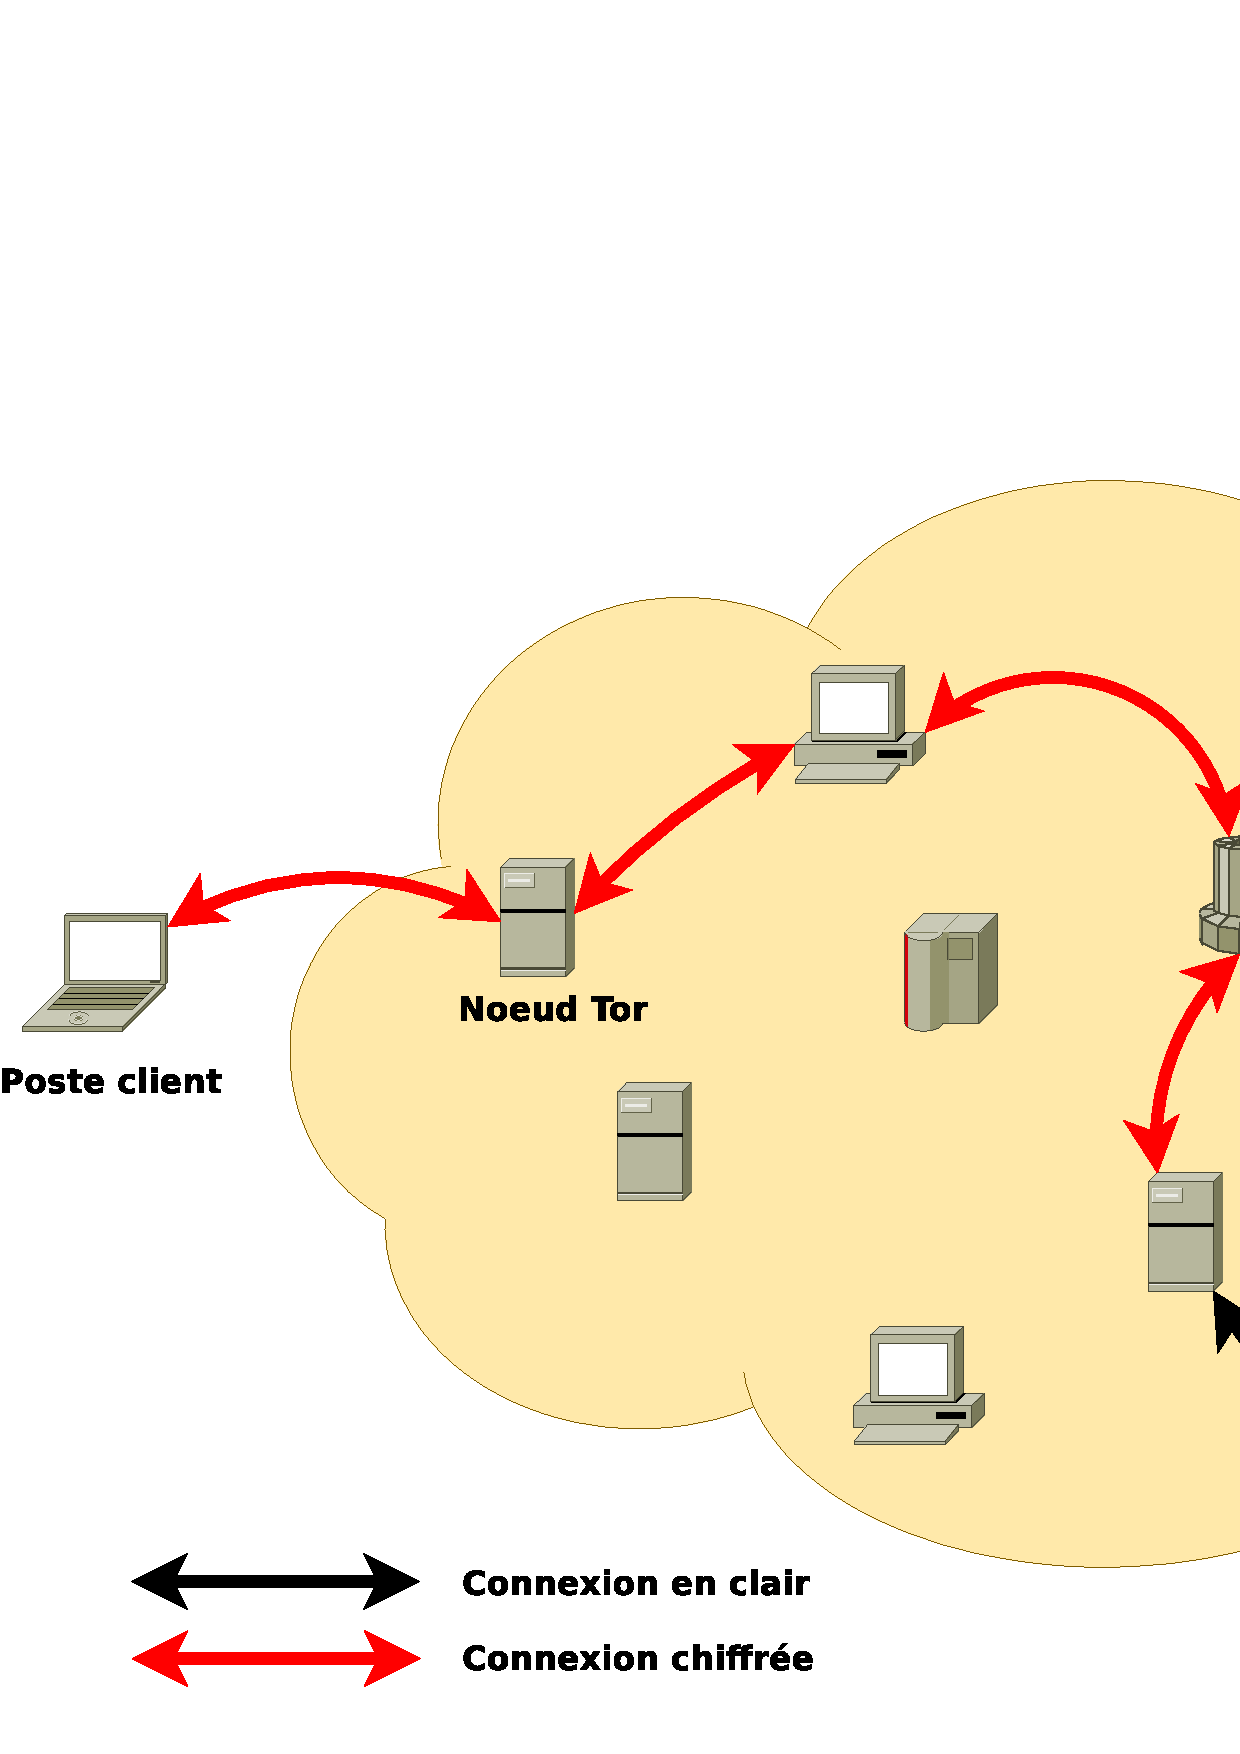
\includegraphics[width=3cm]{inc/tor.png}}
        
        \begin{exampleblock}{Tor = \textit{The Onion Router}}
          Principe~: faire transiter les messages par un certain
          nombre de n\oe uds (machines) choisis au hasard, avant de
          les remettre à leur destinataire, en utilisant des
          chiffrements successifs entre les n\oe uds (chiffrement en
          couches, d'où l'image de l'oignon).

          ~\\
          Objectif poursuivi (à préciser dans la suite)~: protection
          de la vie privée d'un usager du web.
        \end{exampleblock}

        \begin{block}{}
          Tor est un réseau de machines (n\oe uds Tor), avec des n\oe
          uds \og d'entrée\fg\ et \og\ de sortie\fg , que tout le
          monde peut utiliser de cette manière.
        \end{block}
      }
      \frame{
        \frametitle{Présentation de Tor}

        \centerline{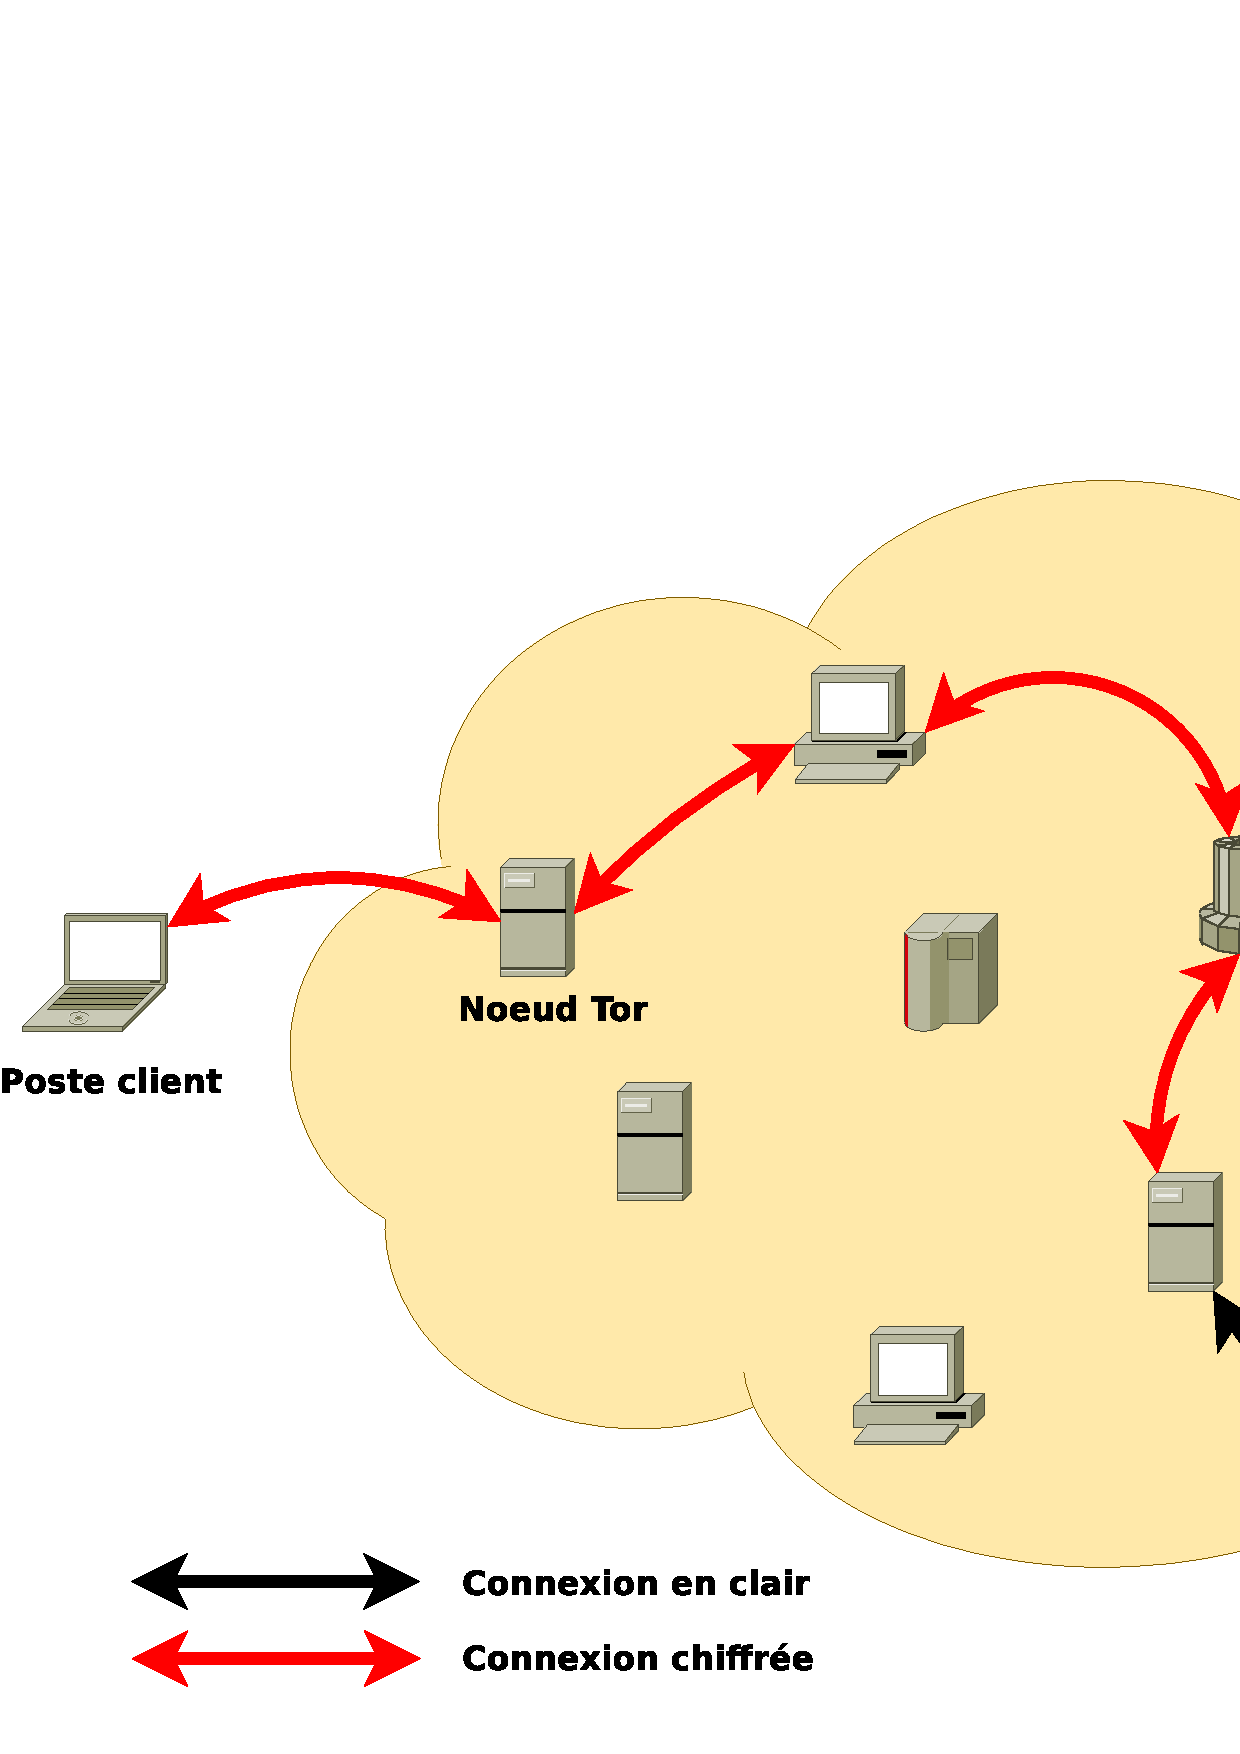
\includegraphics[width=10cm]{inc/tor.pdf}}
      }
      \frame{
        \frametitle{Présentation de Tor}

        \centerline{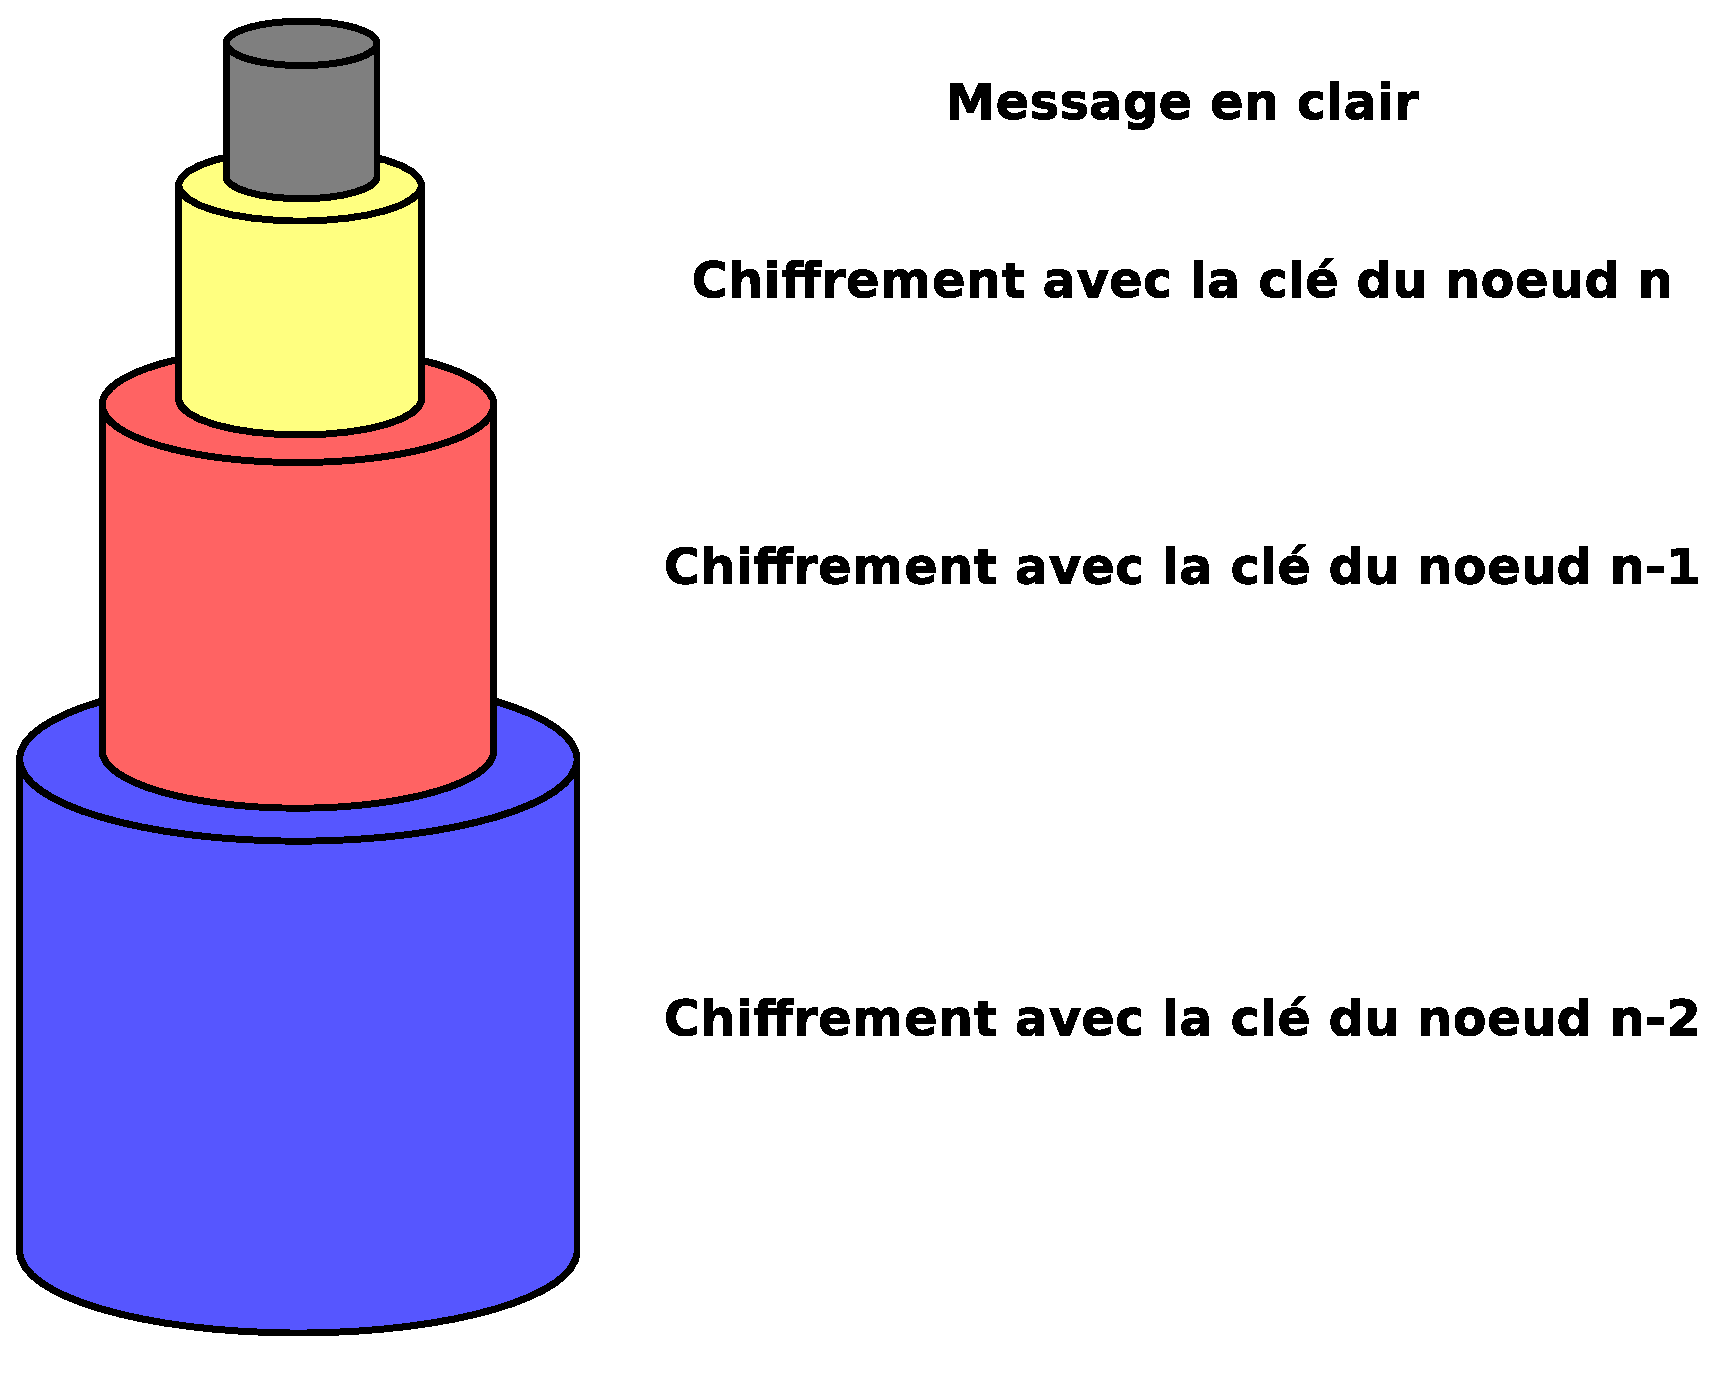
\includegraphics[width=8cm]{inc/oignon}}
      }
      \frame{
        %\frametitle{Le réseau Tor}
        \small

        \begin{block}{Établissement d'un circuit Tor par le n\oe ud
            A~: principe}
          \begin{itemize}
          \item $A$ choisit une séquence de n\oe uds commençant par un
            n\oe ud d'entrée ($B$) et terminant par un n\oe ud de
            sortie, et récupère les clés publiques des n\oe uds du
            circuit~;
          \item $A$ associe en interne à $B$ un nouveau numéro de circuit
            $circID_{AB}$~;
          \item $A$ envoie un message \texttt{create} à $B$, contenant
            $circID_{AB}$ et la première moitié d'un Diffie-Hellman
            chiffrée avec la clé publique de $B$~;
          \item $B$ renvoie un message \texttt{created}, avec la
            deuxième moitié du Diffie-Hellman et le condensat de la
            clé de session $K_{AB}$~;
          \item A envoie un \texttt{relay extend} à $B$ en lui
            désignant $C$ et en transmettant une moitié de
            Diffie-Hellman chiffrée avec la clé publique de $C$~;
          \item $B$ choisit en interne un nouveau numéro de circuit
            $circID_{BC}$, qu'il associe à $circID_{AB}$~;
          \item $B$ transmet le message à $C$ dans un \texttt{create}
            étiqueté $circID_{BC}$~;
          \item $C$ renvoie un message \texttt{created} que $B$
            transmet à $A$ sous la forme d'un \texttt{relay
              extended}~: $A$ et $C$ partagent $K_{AC}$~;
          \item etc.
          \end{itemize}
        \end{block}
      }
      \section{Manipulation en classe}
      \subsection*{~}
      \frame{
        \frametitle{Manipulation en classe}

        \begin{block}{Matériel requis}
          \begin{itemize}
          \item Une classe divisée en 5 groupes A (émetteurs), B (n\oe
            uds d'entrée), C (n\oe uds intermédiaires), D (n\oe uds de
            sortie) et E (destinataires) (par exemple organisés en 5
            rangées)~;
          % \item Une manière pratique et visible de numéroter chaque
          %   participant (A1, A2\ldots, B1, B2\ldots)~;
          \item Des enveloppes de trois tailles rentrant les unes dans
            les autres~;
          \item Des papiers entrant dans les petites enveloppes~;
          \item Papier et gomme pour chacun~;
          \item Les fiches pratiques \og émetteur\fg, \og n\oe ud
            d'entrée\fg, \og n\oe ud intermédiaire\fg, \og n\oe ud de
            sortie\fg, \og destinataire\fg~;
          \item Un peu de concentration\ldots
          \end{itemize}
          
        \end{block}
      }

      \section{Conclusions}
      \subsection*{}
      \frame{
        \frametitle{Le réseau Tor}

        \begin{exampleblock}{Propriétés assurées}
          \begin{itemize}
          \item Anonymisation IP du client, vis-à-vis de tout le monde
            excepté le n\oe ud d'entrée~;
          \item Contenu des messages et destinataire chiffrés jusqu'au
            n\oe ud de sortie (point sensible).
          \end{itemize}
        \end{exampleblock}

        \begin{alertblock}<2>{Mais~!}
          \begin{itemize}
          \item Nécessité d'utiliser un proxy spécifique sur la
            machine client~;
          \item Nécessité de \og torréfier\fg\ les applications~;
          \item Grand temps de latence, inadapté pour les gros volumes
            de données~;
          \item Pas d'anonymisation applicative~: on peut être
            identifié par le contenu des messages~;
          \item Les n\oe uds d'entrée et de sortie sont publics et
            peuvent être interdits d'accès.
          \end{itemize}
        \end{alertblock}
      }
      % \frame{
      %   \frametitle{Le réseau Tor}

      %   \begin{exampleblock}{\textit{Tor hidden services}}
      %     Sites web ou services divers, accessibles uniquement depuis
      %     Tor. Un \textit{hidden service} a une URI en
      %     \texttt{.onion}, mais pas d'adresse IP~: services non
      %     géolocalisables, a priori complètement anonymes.
      %   \end{exampleblock}

      %   \begin{block}{Mise en place d'un \textit{hidden service}}
      %     \begin{enumerate}
      %     \item Le n\oe ud fournisseur du service choisit plusieurs
      %       \textit{points d'introduction} parmi les autres n\oe uds,
      %       leur transmet sa clé publique et établit des circuits avec
      %       eux~;
      %     \item Le n\oe ud de service crée un descripteur incluant sa
      %       clé publique et la liste des points d'introduction, et le
      %       signe~;
      %     \item Le n\oe ud publie le descripteur dans une DHT, sous
      %       une clé \texttt{XXX.onion} où \texttt{XXX} est une chaîne
      %       de 16 caractères dérivée de sa clé publique.
      %     \end{enumerate}
      %   \end{block}
      % }
      % \frame{
      %   %\frametitle{Le réseau Tor}

      %   \begin{block}{Accès à un \textit{hidden service}}
      %     \begin{enumerate}
      %     \item Le client dispose de l'adresse \texttt{XXX.onion} (via
      %       un moteur de recherche par exemple~:
      %       \texttt{http://ahmia.fi/})~;
      %     \item Le client télécharge le descripteur depuis la DHT~;
      %     \item Le client choisit un n\oe ud pour servir de point de
      %       rendez-vous, il établit un circuit et lui envoie un secret
      %       de session~;
      %     \item Le client forge un \textit{message d'introduction},
      %       incluant l'identité du point de RDV et le secret de
      %       session, le tout chiffré avec la clé publique du service~;
      %     \item Le client envoie le message d'introduction à un point
      %       d'introduction (via un circuit Tor), qui le transmet au
      %       n\oe ud de service~;
      %     \item Le n\oe ud de service déchiffre le message
      %       d'introduction et établit un circuit jusqu'au point de
      %       RDV, auprès duquel il s'identifie avec le secret de
      %       session~;
      %     \item Le point de RDV notifie le client, client et n\oe ud
      %       de service peuvent alors communiquer par leurs circuits
      %       respectifs au point de RDV.
      %     \end{enumerate}
      %   \end{block}
      % }
      \section*{}
      \frame{
        \frametitle{Crédits}

        \scriptsize

        \begin{tabular}{m{2.5cm}m{7cm}}
          %\hline
          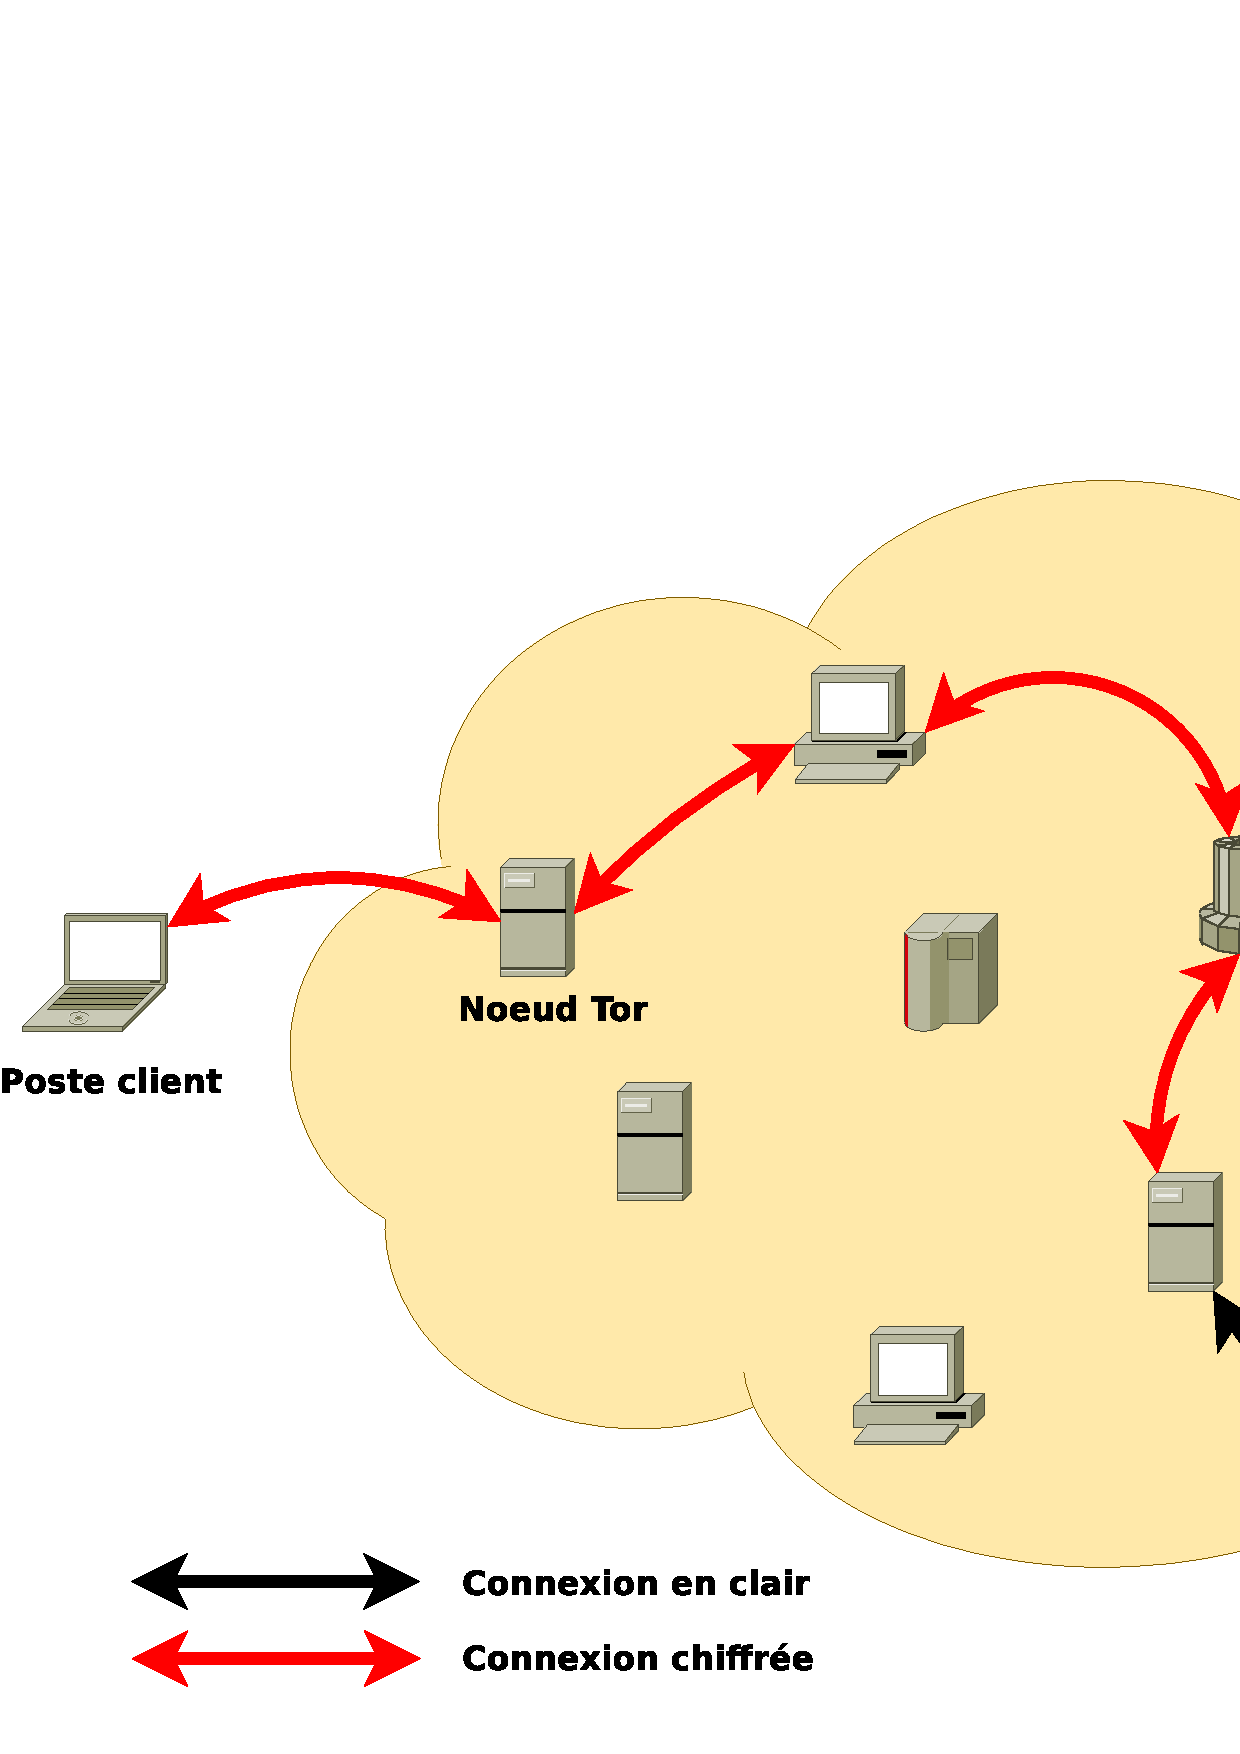
\includegraphics[height=0.3cm]{inc/tor.png} &
          The Tor Project, Inc. (\url{https://www.torproject.org/}), CC-BY 3.0
          \\
        \end{tabular}
        
      }
      
\end{document}

%%% Local Variables:
%%% mode: latex
%%% TeX-master: t
%%% ispell-local-dictionary: "francais"
%%% End: 
